\documentclass{article}


% to compile a camera-ready version, add the [final] option, e.g.:
\usepackage[final]{neurips}

% to avoid loading the natbib package, add option nonatbib:
    % \usepackage[nonatbib]{neurips_2019}

\usepackage[utf8]{inputenc} 	% allow utf-8 input
\usepackage[T1]{fontenc}    		% use 8-bit T1 fonts
\usepackage{hyperref}       		% hyperlinks
\usepackage{url}            		% simple URL typesetting
\usepackage{booktabs}       		% professional-quality tables
\usepackage{amsfonts}       		% blackboard math symbols
\usepackage{nicefrac}       		% compact symbols for 1/2, etc.
\usepackage{microtype}      		% microtypography
%\usepackage{breqn}			% dmath
\usepackage{listings}
\usepackage{amsmath}     		% multiline
\usepackage{graphicx}
\usepackage{xepersian}
\usepackage{graphicx}



\settextfont{XB Niloofar.ttf}

\title{پاسخ تمرین سری ۱ }




\author{%
  محمدرضا عزیزی\\
  ۹۸۱۳۱۰۲۲ \\
  دانشکده مهندسی کامپیوتر\\
  دانشگاه صنعتی امیرکبیر (پلی‌تکنیک تهران)\\
  \texttt{mrazizi@aut.ac.ir} \\
}


\renewcommand{\baselinestretch}{1.5} 

\begin{document}


\begin{minipage}{0.1\textwidth}% adapt widths of minipages to your needs

\includegraphics[width=1.1cm]{aut_logo.png}
\end{minipage}%
\hfill%
\begin{minipage}{0.9\textwidth}\raggedleft
دانشگاه صنعتی امیرکبیر (پلی‌تکنیک تهران)\\
شبکه‌های عصبی (بهار ۱۳۹۹)\\
\end{minipage}
% \end{}


\makepertitle




% 1
\section{
راهکاری برای پیش‌پردازش داده‌ها
}

داده‌ها با استفاده از کتابخانه pandas بارگذاری کرده و از آن‌جایی که ستون‌های داده‌ها نام ندارد، ابتدا با توجه به توضیحات دیتاست، یک لیست برای نام ستون‌ها تعریف کرده و این نام‌ها را به ستون‌های دیتافریم بارگذاری شده اضافه می‌کنیم. لیست این نام‌ها به ترتیب برابر است با:

\begin{latin}
\begin{lstlisting}
["age", "workclass", "fnlwgt", "education", "education-num", 
"marital-status", "occupation", "relationship", "race", "sex", 
"capital-gain", "capital-loss", "hours-per-week", "native-country", "label"]
\end{lstlisting}
\end{latin}

ستون آخر که مربوط به برچسب داده‌است با با نام label نام‌گذاری کرده‌ایم. \\

راه حلی که در ابتدا ممکن است به ذهن برسد این است که یک دیکشنری تعریف کنیم که هر دوتایی کلید/مقدار آن، خود یک دیکشنری است. برای مثال به ازای کلید label، دیکشنری زیر را داریم:

\begin{latin}
\begin{lstlisting}
'label': {'<=50K':0, '>50K': 1}
\end{lstlisting}
\end{latin}

به ازای تمامی مقادیر تمامی ستون‌هایی که مقدار عددی ندارند، این دیکشنری را تعریف کرده و به هر مقدار اسمی، یک عدد نسبت دهیم. این اعداد از برای هر متغیر از ۰ شروع شده و یک واحد یک واحد افزایش می‌یابد. 

در نهایت با استفاده از تابع replace از کتابخانه pandas، طبق دیکشنری تعریف شده، مقادیر اسمی را به مقادیر عددی تبدیل کنیم. \\

در ابتدا روش ذکر شده را پیاده‌سازی کردیم و بارگذاری داده به صورت زیر بود:

\begin{center}
	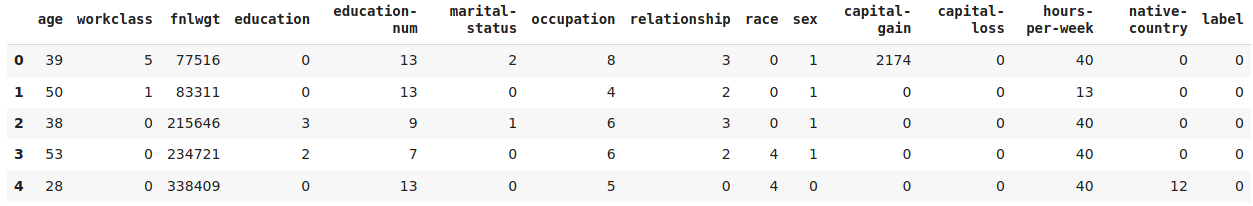
\includegraphics[scale=0.35]{df_numeric.png} 
\end{center}    

اما این روش کدگذاری داده‌های اسمی یک مشکل بزرگ دارد. برای مثال به کدگذاری متغیر relationship دقت کنید:


\begin{latin}
\begin{lstlisting}
'relationship': {'Wife':0, 'Own-child':1, 'Husband':2, 'Not-in-family':3,
                     'Other-relative':4, 'Unmarried':5},
\end{lstlisting}
\end{latin}

در این حالت به یک فرد که ازدواج نکرده‌ است عدد ۵ نسبت داده می‌شود. به یک فرد که نقش شوهر دارد عدد ۲ و به فردی که نقش زن دارد، عدد ۰، در حالی که به وضوح در دیتاست این مساله، هیچ تناسبی بین این افراد وجود ندارد. یعنی رابطه‌ای از این جهت که فرد ازدواج نکرده فاصله‌ عددش با زن یا شوهر چقدر باید باشد، وجود ندارد. \\

بنابراین از ادامه دادن مساله با این روش منصرف شده و در ادامه به سراغ روش \lr{One hot encoding} می‌رویم.

قبل از کدگذاری با استفاده از این روش، باید راه‌حلی برای داده‌های گم‌شده پیدا کنیم. در این مساله، ما برای داده‌های عددی، میانگین هر ستون را جایگزین مقدار گم‌شده کرده و برای داده‌های اسمی، مقداری که بیشترین تکرار را دارد جایگزین مقدار گم‌شده می‌کنیم. این کار با استفاده از کلاس DataFrameImputer انجام شده‌است. \\

می‌دانیم که \lr{one hot encoding} به این صورت است که به ازای هر مقدار یک متغیر، یک ستون جدید ایجاد می‌شود و ردیف‌هایی که آن مقدار را دارند، در آن ستون ۱ و در دیگر ستون‌ها مقدار ۰ خواهند گرفت. ستون‌هایی از دیتافریم را که نیاز به تبدیل شدن به \lr{one hot} دارند به عنوان ورودی به تابع \lr{get\_dummies} از کتابخانه pandas می‌دهیم. ورودی‌ها را انتخاب کرده و برای خروجی نیز صرفا یکی از ستون‌های مربوط به «بیشتر بودن درآمد از ۵۰ هزار دلار» یا «کمتر مساوی بودن درآمد با ۵۰ هزار دلار» را انتخاب می‌کنیم. دلیل این کار این است که هر گاه مقدار ستون اولی برای یک ردیف برابر با یک باشد، مقدار آن ردیف در ستون دوم برابر با صفر است و برعکس. \\

یکی دیگر از مراحل پیش‌پردازش، نرمال کردن داده‌ها است. نرمال کردن داده‌ها با این هدف انجام می‌شود که همه مقادیر بین ۰ تا ۱ باشند و ناخواسته تاثیر یک ستون (ویژگی) بیشتر از ستون دیگری در نظر گرفته نشود.



% add page break after each section
\let\oldsection\section
\renewcommand\section{\clearpage\oldsection}



%%%%%%%%%%%%%%%%%%%%%%%%%%%%%%%%%%%%%%%%%%%%%%%%%%


% 2
\section{
بارگذاری داده‌ها و انجام پیش‌پردازش
}


پس از بارگذاری داده‌ها و انجام پیش‌پردازش‌های ذکرشده در بخش ۱، ستون \lr{label\_>50K} را به عنوان label در نظر گرفته و بقیه ستون‌های سمت چپ را به عنوان ورودی شبکه عصبی در نظر می‌گیریم.

ابعاد ورودی و خروجی نهایی ما به صورت زیر خواهد بود:


\begin{latin}
\begin{lstlisting}
x_train shape: (32561, 105)
y_train shape: (32561,)
\end{lstlisting}
\end{latin}

مجموعا ۳۲۵۶۱ داده داریم (که در آینده به عنوان داده آموزش و ارزیابی استفاده خواهد شد) و هر داده، ۱۰۵ بعد (یا ویژگی) دارد.



%%%%%%%%%%%%%%%%%%%%%%%%%%%%%%%%%%%%%%%%%%%%%%%%%%

% 3
\section{
طراحی مدل
}

برای طراحی مدل، می‌دانیم لایه ورودی، باید به اندازه شکل داده‌های ما نورون داشته باشد، بنابراین از shape متغیر \lr{x\_train} به عنوان شکل ورودی تابع استفاده می‌کنیم. همچنین می‌دانیم که در لایه آخر می‌توانیم صرفا یک نورون داشته باشیم که با یک تابع فعال‌سازی sigmoid مقدار دو کلاس را مشخص می‌کند.

تابع ارزیابی تمامی لایه‌های میانی را نیز برابر relu انتخاب می‌کنیم.

برای انتخاب بهترین مدل و بهترین مقادیر هایپرپارامترها، ۲۰ درصد از داده‌های آموزشی را جدا کرده و به عنوان داده ارزیابی در نظر می‌گیریم. با ساختارهای مختلف شبکه و مقادیر هایپرپارامتر مختلف، شبکه را آموزش داده و بر اساس مقدار  loss مربوط به داده ارزیابی بهترین ساختار را انتخاب می‌کنیم. \\

طبق درخواست بخش ۵ صورت سوال، از بهینه‌ساز Adam و تابع هزینه \lr{binary crossentrpy} (به دلیل وجود دو کلاس دسته‌بندی) برای بهینه‌سازی مدل خود استفاده می‌کنیم. \\

انتخاب ساختار شبکه عصبی بر اساس آزمون و خطا است. در تمامی آزمون‌ها از تابع فعال‌سازی relu در لایه‌های میانی و از تابع فعال‌سازی sigmoid در لایه پایانی استفاده می‌کنیم. دلیل استفاده از تابع relu این است که به طور کلی مشاهده شده است که در مسائل مختلف، نتیجه بهتری می‌دهد. دلیل استفاده از تابع فعال‌سازی sigmoid در لایه‌ آخر این است که نیاز داریم که خروجی بین ۰ و ۱ باشد. در رابطه با تعداد لایه‌ها و تعداد نورون‌های هر لایه، آزمایش‌هایی انجام داده‌ایم که به شرح زیر است:



آزمون ۱:

\begin{latin}
\begin{lstlisting}
_________________________________________________________________
Layer (type)                 Output Shape              Param #   
=================================================================
dense_12 (Dense)             (None, 128)               13568     
_________________________________________________________________
dense_13 (Dense)             (None, 1)                 129       
=================================================================
Total params: 13,697
Trainable params: 13,697
Non-trainable params: 0
_________________________________________________________________
\end{lstlisting}
\end{latin}


\begin{latin}
\begin{lstlisting}
----- Training -----
loss: 0.2734 / accuracy: 0.8729 / precision: 0.765 / recall: 0.6775 /
f1_score = 0.6885

Confusion Matrix - for train:
TP = 4228.0 	 FP = 1298.0
FN = 2013.0 	 TN = 18509.0


----- Validation -----
loss: 0.3252 / accuracy: 0.8554 / precision: 0.7232 / recall: 0.6662 /
f1_score = 0.6799

Confusion Matrix - for validation:
TP = 1066.0 	 FP = 408.0
FN = 534.0 	 TN = 4505.0
\end{lstlisting}
\end{latin}

\bigbreak

آزمون ۲:

\begin{latin}
\begin{lstlisting}
_________________________________________________________________
Layer (type)                 Output Shape              Param #   
=================================================================
dense_14 (Dense)             (None, 512)               54272     
_________________________________________________________________
dense_15 (Dense)             (None, 1)                 513       
=================================================================
Total params: 54,785
Trainable params: 54,785
Non-trainable params: 0
_________________________________________________________________
\end{lstlisting}
\end{latin}

\begin{latin}
\begin{lstlisting}
----- Training -----
loss: 0.2835 / accuracy: 0.8684 / precision: 0.7566 / recall: 0.6645 /
f1_score = 0.7076

Confusion Matrix - for train:
TP = 4147.0 	 FP = 1334.0
FN = 2094.0 	 TN = 18473.0


----- Validation -----
loss: 0.3238 / accuracy: 0.8537 / precision: 0.7273 / recall: 0.6469 / 
f1_score = 0.6847

Confusion Matrix - for validation:
TP = 1035.0 	 FP = 388.0
FN = 565.0 	 TN = 4525.0
\end{lstlisting}
\end{latin}

\bigbreak


آزمون ۳:

\begin{latin}
\begin{lstlisting}
_________________________________________________________________
Layer (type)                 Output Shape              Param #   
=================================================================
dense (Dense)                (None, 1000)              106000    
_________________________________________________________________
dense_1 (Dense)              (None, 20)                20020     
_________________________________________________________________
dense_2 (Dense)              (None, 1)                 21        
=================================================================
Total params: 126,041
Trainable params: 126,041
Non-trainable params: 0
_________________________________________________________________
\end{lstlisting}
\end{latin}

\begin{latin}
\begin{lstlisting}
----- Training -----
loss: 0.2700 / accuracy: 0.8738 / precision: 0.7683 / recall: 0.6779 /
f1_score = 0.7203

Confusion Matrix - for train:
TP = 4231.0 	 FP = 1276.0
FN = 2010.0 	 TN = 18531.0


----- Validation -----
loss: 0.3274 / accuracy: 0.8534 / precision: 0.7391 / recall: 0.6231 /
f1_score = 0.6762

Confusion Matrix - for validation:
TP = 997.0 	 FP = 352.0
FN = 603.0 	 TN = 4561.0
\end{lstlisting}
\end{latin}

\bigbreak

آزمون ۴:

آزمون ۱ مقدار accuracy بالاتری دارد و آزمون ۲ مقدار امتیاز f1 بالاتری. مقدار بیشتر بودن امتیاز آزمون ۲ در حد ۱ صدم است و بهتر است به خاطر ۱ صدم، پیچیدگی مدل را چندین برابر نکنیم؛ زیرا همان طور که مشاهده می‌شود آزمون ۱ حدود ۱۳ هزار پارامتر و آزمون ۲ حدود ۵۴ هزار پارامتر دارد. پس مدل ۱ را بهترین مدل در نظر می‌گیریم.

مدل آزمون ۱ را با تابع فعال‌سازی tanh برای لایه میانی، آموزش دادیم و نتایج به صورت زیر بود:

\begin{latin}
\begin{lstlisting}
----- Training -----
loss: 0.3011 / accuracy: 0.8607 / precision: 0.7466 / recall: 0.6336 / 
f1_score = 0.6854

Confusion Matrix - for train:
TP = 3954.0 	 FP = 1342.0
FN = 2287.0 	 TN = 18465.0


----- Validation -----
loss: 0.3199 / accuracy: 0.8503 / precision: 0.7181 / recall: 0.6431 / 
f1_score = 0.6785

Confusion Matrix - for validation:
TP = 1029.0 	 FP = 404.0
FN = 571.0 	 TN = 4509.0
\end{lstlisting}
\end{latin}

\bigbreak


آزمون‌های دیگر:

در آزمون‌های دیگری، ضریب یادگیری را تغییر دادیم و بیش از این تعداد لایه‌ها و نورون‌ها را تغییر دادیم ولی نتیجه بهبود نیافت و از آوردن آن آزمایش‌ها در گزارش صرف نظر شده است.\\ 

مشاهده می‌شود که رسیدن به دقت حدود ۸۵ درصد برای مساله چندان مشکل نیست و با افزایش تعداد نورون‌های لایه میانی یا افزایش تعداد لایه‌ها، مساله بهبود پیدا نمی‌کند. بنابر اصل تیغ اوکام، ساده‌ترین مدل - که در اینجا بهترین نتیجه بر روی داده‌های ارزیابی را نیز به دست آورده است - را انتخاب می‌کنیم. (مدل آزمون اول)

با انتخاب این هایپرپارامترها و آموزش مدل برای ۱۰ epoch ، دقت مدل بر روی داده‌های ارزیابی به ۸۶ درصد و بر روی داده‌های آموزش به ۸۷ درصد رسید. \\

ساختار مدل:



\begin{center}
	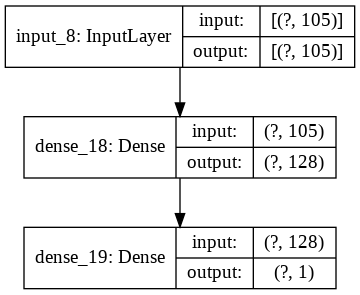
\includegraphics[scale=0.45]{model.png} 
\end{center}    



\begin{latin}
\begin{lstlisting}
Hyperparameters:
Optimizer: Adam (lr = 0.0005)
loss: binary crossentropy
epochs: 10
shuffle: True
\end{lstlisting}
\end{latin}


\begin{latin}
\begin{lstlisting}
loss: 0.2874
accuracy: 0.8665
val_loss: 0.3137
val_accuracy: 0.8575
\end{lstlisting}
\end{latin}

%%%%%%%%%%%%%%%%%%%%%%%%%%%%%%%%%%%%%%%%%%%%%%%%%%

% 4
\section{
تصویر گراف مدل توسط Tensorboard
}

برای استفاده از Tensorboard، یک callback برای آن ساخته و در هنگام اجرای تابع fit، آن را به عنوان ورودی به تابع پاس می‌دهیم.

پس از اجرای Tensorboard، باید دقت شود که تمامی مدل‌هایی که از ابتدای این session نرم‌افزار \lr{Google Colab} ساخته و آموزش داده شده است،‌ نمایش داده ‌می‌شود. مدل مورد نظر ما، آخرین مدل ساخته شده است. می‌توان با ریست کردن session تنها یک مدل را نمایش داد.

\begin{center}
	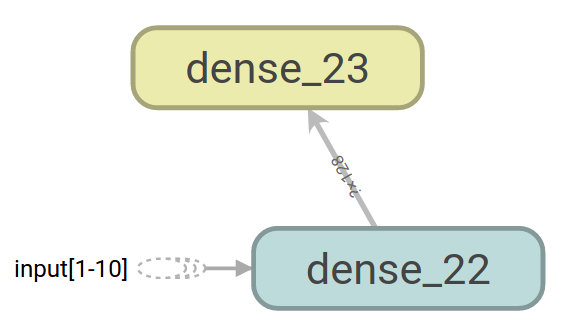
\includegraphics[scale=0.45]{model_graph.png} 
\end{center}    

نمودارهای نحوه کاهش دقت و مقدار تابع زیان هم به صورت زیر است.
در نمودارهای زیر، محور افقی، شماره epoch و محور عمودی مقدار دقت (در نمودار اول) و مقدار تابع زیان (در نمودار دوم) است. همچنین خطوط نارنجی رنگ مربوط به داده آموزش و خطوط آبی مربوط به داده ارزیابی است.


\begin{center}
	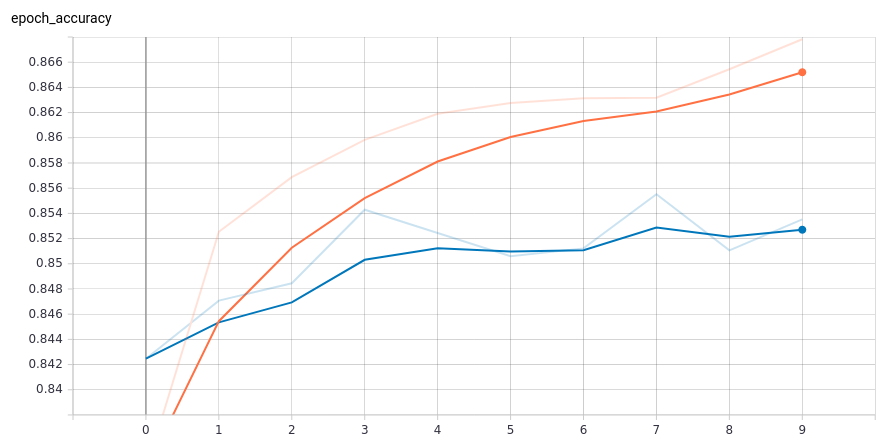
\includegraphics[scale=0.45]{epoch_accuracy.png} 
\end{center}    

\begin{center}
	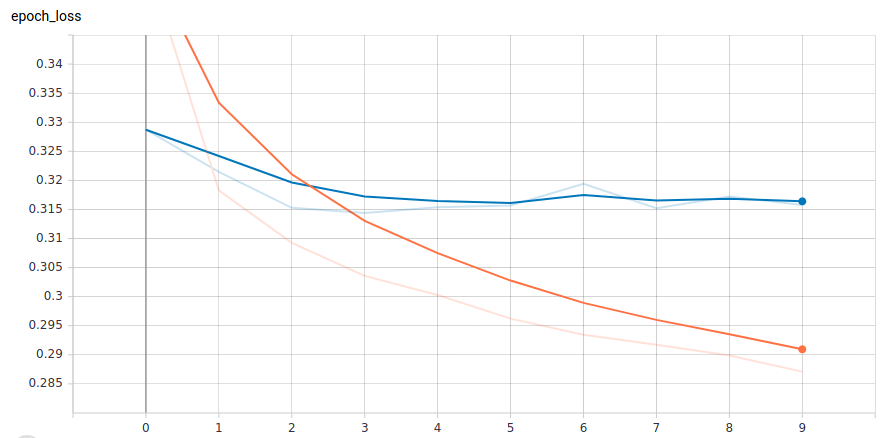
\includegraphics[scale=0.45]{epoch_loss.png} 
\end{center}    


%%%%%%%%%%%%%%%%%%%%%%%%%%%%%%%%%%%%%%%%%%%%%%%%%%
% 5
\section{
بهینه‌ساز مدل و معیارهای ارزیابی
}

بهینه‌ساز Adam و تابع هزینه \lr{Binary CrossEntrophy} - همان‌طور که در بخش ۳ توضیح داده‌شد - انتخاب شده است. \\

تمامی معیارهای ارزیابی مدل، در مجموعه معیارهای تنسورفلو وجود دارد. برای معیار ماتریس درهم‌ریختگی نیز، ۴ معیار TP، FP و TN و TP را از مدل گرفته و کنار هم قرار می‌دهیم. تمامی این مقادیر به ازای هر آزمایش، در بخش ۳ داکیومنت نوشته شده است.

%%%%%%%%%%%%%%%%%%%%%%%%%%%%%%%%%%%%%%%%%%%%%%%%%%

% 6
\section{
تقسیم داده‌ها به سه دسته
}

تا به اینجا، فایل \lr{adult.data} را بارگذاری کرده بودیم و ۸۰ درصد این فایل را به عنوان داده آموزش و ۲۰ درصد را به عنوان داده ارزیابی در نظر گرفته بودیم.

برای داده‌ تست، فایل \lr{adult.test} را بارگذاری می‌کنیم و تمامی پیش‌‌پردازش‌هایی که بر روی داده قبلی انجام داده بودیم، بر روی این مجموعه داده نیز انجام می‌دهیم.


دو نکته در بارگذاری این دیتاست تست وجود دارد. قبل از بارگذاری، خط اول دیتاست که اطلاعاتی است که مربوط به دادگان نیست را به صورت دستی پاک کرده‌ایم. همچنین در دیتاست تست، بعد از مقادیر label، نقطه وجود دارد که این نقاط را نیز با استفاده از تابع replace کتابخانه pandas پاک کرده‌ایم.


وقتی با استفاده از تابع \lr{get\_dummies} از کتابخانه pandas عمل تبدیل دیتافریم تست به کد \lr{one hot} را انجام می‌دهیم، می‌بینیم که تعداد ستون‌های ایجاد شده برابر با ۱۰۶ ستون است، در حالی که تعداد ستون‌های ایجاد شده از داده‌های آموزشی برابر با ۱۰۷ ستون است. دلیل این اتفاق این است که داده‌های تست، یکی از مقادیر یکی از ستون‌های اسمی را ندارند. در این حالت نمی‌توان ورودی را به شبکه عصبی داد. 

باید ابتدا به دنبال ستونی که موجود نیست بگردیم. برای این کار، لیست ستون‌های دیتافریم آموزشی و دیتافریم تست را با هم مقایسه می‌کنیم. مشاهده می‌کنیم که ستونی با نام \lr{native-country\_Holand-Netherlands} در دیتافریم تست در مکان شماره ۷۸ وجود ندارد. این به این معنی است که هیچ‌ داده‌ای با این مقدار وجود ندارد. یک ستون با این نام و در همین مکان به دیتافریم تست اضافه می‌کنیم و در نهایت بررسی می‌کنیم که شکل دو دیتافریم تست و آموزش مشابه هم باشد:


\begin{latin}
\begin{lstlisting}
test df: (16281, 107)
train df: (32561, 107)
\end{lstlisting}
\end{latin}

در بخش در رابطه با آموزش شبکه با استفاده از داده‌های آموزش و بررسی کیفیت عملکرد شبکه در هر epoch توسط داده‌های ارزیابی صحبت شد. تعداد epoch آموزش برابر ۱۰ قرار گرفته است که با توجه به نمودارهایی که در بخش ۴ آورده شده است، مشاهده می‌شود که تغییرات دقت و مقدار تابع زیان برای داده‌های ارزیابی تقریبا به ۰ رسیده است. یعنی شبکه به اندازه کافی آموزش دیده است.




%%%%%%%%%%%%%%%%%%%%%%%%%%%%%%%%%%%%%%%%%%%%%%%%%%

% 7
\section{
evaluate
}

%%%%%%%%%%%%%%%%%%%%%%%%%%%%%%%%%%%%%%%%%%%%%%%%%%

% 4
\section{
تصویر گراف مدل توسط Tensorboard
}

%%%%%%%%%%%%%%%%%%%%%%%%%%%%%%%%%%%%%%%%%%%%%%%%%%

% 4
\section{
تصویر گراف مدل توسط Tensorboard
}

%\section*{منابع}

\medskip

\small
\LTR 
\latin



\end{document}
